\documentclass{article}
\usepackage{graphicx}
\graphicspath{ {/} }

\begin{document}
\title{A research done on the different age brackets in makerere to find out  their locations}
\author{kyalisiima nicholas}

\maketitle

\begin{abstract}
The document is to show the results that were attained from the research carried out in campus to get the locations of the people at campus .
\end{abstract}

\section{Introduction}
The research aimed at figuring out where different people in makerere are located.

\subsection{The Kind of data collected}
\begin{itemize}
\item{I made a form that requires the user to enter his name, age,location , photo of the user .}
\item{I moved around the university and took data from a number of people around the campus}
\item{After I had got the data, I made a table showing the data that has been collected and then I used it to make a visualization of the data.} 
\end{itemize}

\subsection{Time it was collected}
\begin{itemize}
\item{The data was collected during the times of midday to 6pm because those are the times that I was able to get the attention of people}
\end{itemize}

\subsection{challenges faced}
\begin{itemize}
\item{Some people didn’t want to share their information thinking I was a fraud.}
\item{Sometimes I collect data in a place without strong internet and I had to wait until I had internet connection so that am able to send the data to the server which would delay my updating of the information.}
\item{I wasn’t able to get a big number of people that shared their information with me.}
\item{I had problems setting up the aggregate server which would host my information because I had weak internet that would not successfully make a complete connection to the server.}
\end{itemize}

\subsection{solution of some of the problems}
\begin{itemize}
\item{I got information from people in the area where there was internet connection to make my data update time is quickly}
\end{itemize}

\section{Visualization of data}
After collecting data from people, i was able to make a visualization of the percentage of people whose age i collected,and the current locations.

\subsection{Table  of the data collected}
\begin{tabular}{ |p{3cm}||p{3cm}|p{3cm}|p{3cm}|  }
 \hline
 \multicolumn{4}{|c|}{ Sample of User Data about peoples locations} \\
 \hline
 First Name  & Last Name & age & Location\\
 \hline
 Grace  & Nicolaus    & 22 & MUK\\
 Dickson&   Obenamukama  & 21   &MUK\\
 Bamuhaira &Tracy & 19&  MUK\\
 Ssaka    &Charles & 21&  MUK\\
 James&  Jesus  & 25& MUK\\
 Kiwalabye & Ibrahim & 22  &MUK\\
 \hline
\end{tabular}


\subsection{A piechart showing the location of the people according to their ages }
The different colours show the current location of the people ,and the numbers show the different age brackets.


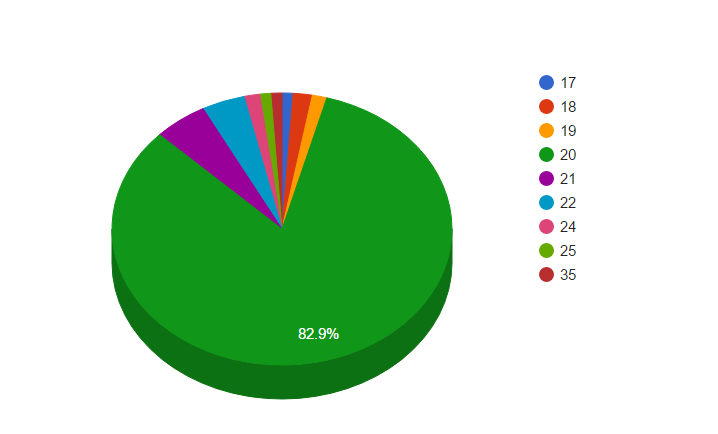
\includegraphics[width=10cm, height=7cm]{pie.PNG}



\subsection{Snapshots of the application used to collect data}

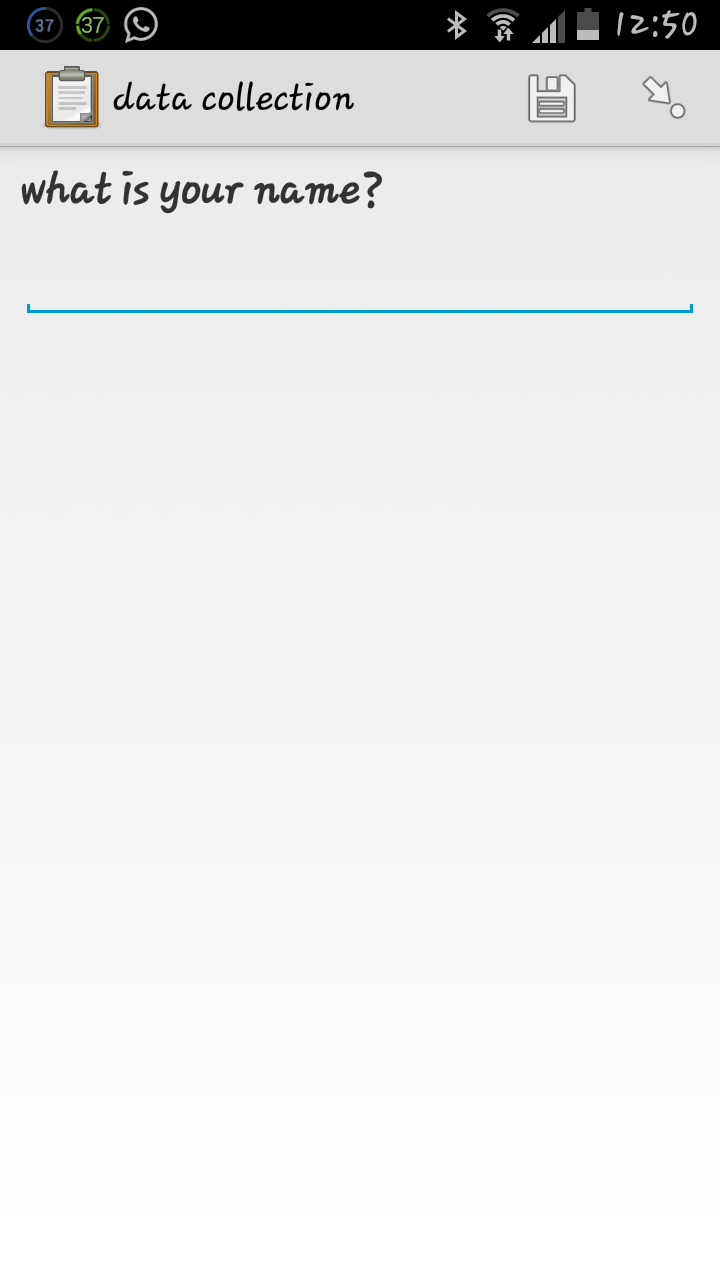
\includegraphics[width=3cm, height=4cm]{test.png}
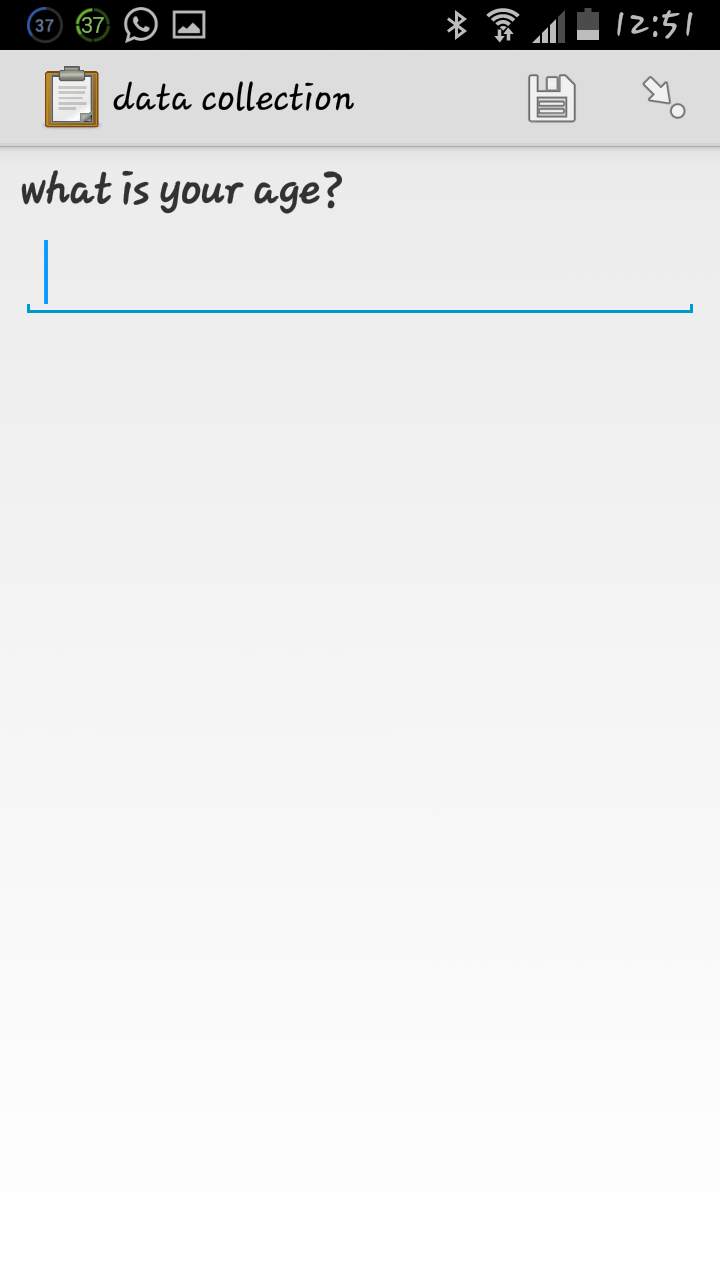
\includegraphics[width=3cm, height=4cm]{test2.png}
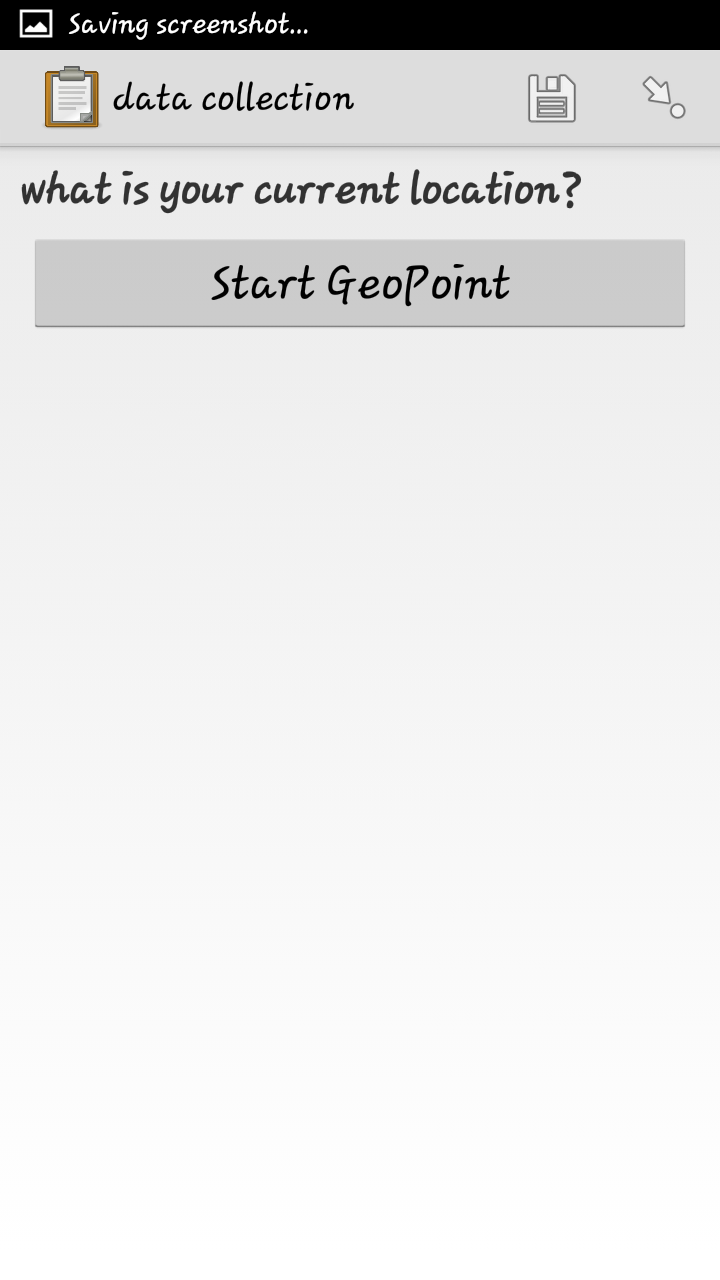
\includegraphics[width=3cm,height=4cm]{test3.png}
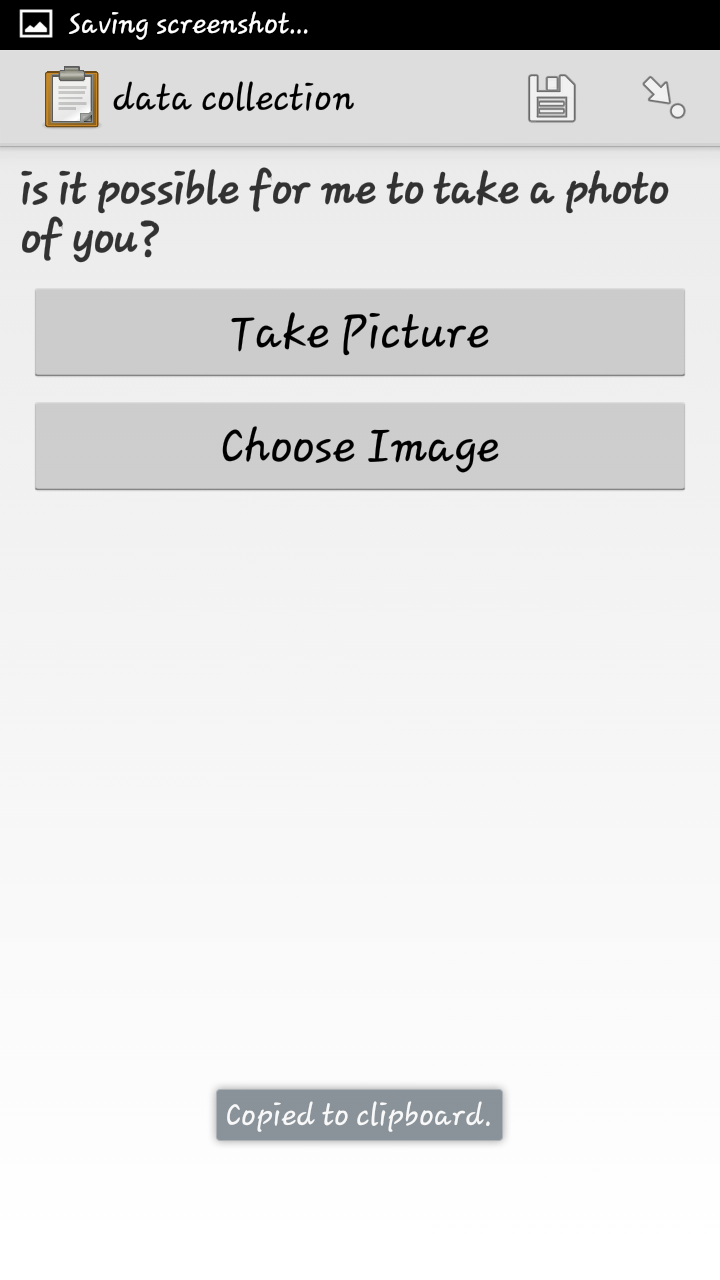
\includegraphics[width=3cm,height=4cm]{test4.png}



\section{Conclusion}
After collecting data in the small area that i was in. I came to a realisation that many of the people in that area are aged 25 years. For some few their reasion was that the place was to expensive for their age brackets to afford the cost of living in the place.

The data that i collected was not in a big area but i was able to get information.
\end{document}
